\documentclass[a4paper, 11pt]{article}
\usepackage{graphicx}
\usepackage{multicol}
\usepackage{tabularx}
\usepackage{enumitem}
\usepackage[a4paper, margin=1.8cm]{geometry}
\usepackage{listings}
\usepackage{amssymb}
\usepackage{gvv}
\usepackage{gvv-book}
\usepackage{amsmath}
\usepackage{setspace}
\usepackage{caption}
\usepackage{tfrupee}
\usepackage{float}

\graphicspath{./figs}

\begin{document}
\begin{center}
    \huge{EC : ELECTRONICS AND COMMUNICATION ENGINEERING}\\
    \large{EE25BTECH11041 - Naman Kumar}
\end{center}

\begin{enumerate}
    \section*{General Aptitude (GA)}
    \item The untimely loss of life is a cause of serious global concern as thousands of people get killed \underline{\hspace{2cm}} accidents every year while many other die \underline{\hspace{2cm}} diseases like cardio vascular disease, cancer, etc.
    \begin{enumerate}
        \begin{multicols}{2}
            \item in, of
            \item from, of
            \item during, from
            \item from, from
        \end{multicols}
    \end{enumerate}

    \hfill{\brak{\text{GATE EC 2020}}}

    \item He was not only accused of theft \underline{\hspace{2cm}} of conspiracy.
    \begin{enumerate}
        \begin{multicols}{2}
            \item rather
            \item but also
            \item but even
            \item rather than
        \end{multicols}
    \end{enumerate}

    \hfill{\brak{\text{GATE EC 2020}}}

    \item Select the word that fits the analogy:
    
    Explicit: Implicit :: Express: \underline{\hspace{2cm}}
    \begin{enumerate}
        \begin{multicols}{2}
            \item Impress
            \item Repress
            \item Compress
            \item Suppress
        \end{multicols}
    \end{enumerate}

    \hfill{\brak{\text{GATE EC 2020}}}

    \item The Canadian constitution requires that equal importance be given to English and French. Last year, Air Canada lost a lawsuit, and had to pay a six-figure fine to a French-speaking couple after they filed complaints about formal in-flight announcements in English lasting 15 seconds, as opposed to informal 5 second messages in French.\\The French-speaking couple were upset at
    \begin{enumerate}
        \item the in-flight announcements being made in English.
        \item the English announcements being clearer than the French ones.
        \item the English announcements being longer than the French ones.
        \item equal importance being given to English and French.
    \end{enumerate}

    \hfill{\brak{\text{GATE EC 2020}}}

    \item A superadditive function $f(\cdot)$ satisfies the following property
    $$f(x_1+x_2) \ge f(x_1)+f(x_2)$$
    Which of the following functions is a superadditive function for $x>1$?
    \begin{enumerate}
        \begin{multicols}{2}
            \item $e^x$
            \item $\sqrt{x}$
            \item $\frac{1}{x}$
            \item $e^{-x}$
        \end{multicols}
    \end{enumerate}

    \hfill{\brak{\text{GATE EC 2020}}}

    \item The global financial crisis in 2008 is considered to be the most serious world-wide financial crisis, which started with the sub-prime lending crisis in USA in 2007. The sub-prime lending crisis led to the banking crisis in 2008 with the collapse of Lehman Brothers in 2008. The sub-prime lending refers to the provision of loans to those borrowers who may have difficulties in repaying loans, and it arises because of excess liquidity following the East Asian crisis.\\Which one of the following sequences shows the correct precedence as per the given passage?
    \begin{enumerate}
        \item East Asian crisis $\rightarrow$ subprime lending crisis $\rightarrow$ banking crisis $\rightarrow$ global financial crisis.
        \item Subprime lending crisis $\rightarrow$ global financial crisis $\rightarrow$ banking crisis $\rightarrow$ East Asian crisis.
        \item Banking crisis $\rightarrow$ subprime lending crisis $\rightarrow$ global financial crisis $\rightarrow$ East Asian crisis.
        \item Global financial crisis $\rightarrow$ East Asian crisis $\rightarrow$ banking crisis $\rightarrow$ subprime lending crisis.
    \end{enumerate}

    \hfill{\brak{\text{GATE EC 2020}}}

    \item It is quarter past three in your watch. The angle between the hour hand and the minute hand is
    \begin{enumerate}
        \begin{multicols}{2}
            \item $0\degree$
            \item $7.5\degree$
            \item $15\degree$
            \item $22.5\degree$
        \end{multicols}
    \end{enumerate}

    \hfill{\brak{\text{GATE EC 2020}}}
    
    \item A circle with centre O is shown in the figure. A rectangle PQRS of maximum possible area is inscribed in the circle. If the radius of the circle is a, then the area of the shaded portion is
    \begin{figure}[H]
        \centering
        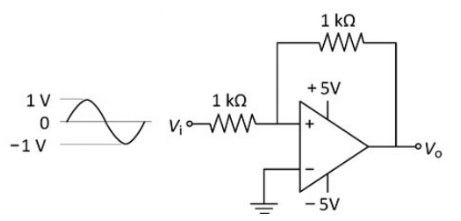
\includegraphics[width=0.3\columnwidth]{figs/Q8.png}
        \caption*{}
        \label{fig:q8}
    \end{figure}
    \begin{enumerate}
        \begin{multicols}{2}
            \item $\pi a^2 - a^2$
            \item $\pi a^2 - \sqrt{2}a^2$
            \item $\pi a^2 - 2a^2$
            \item $\pi a^2 - 3a^2$
        \end{multicols}
    \end{enumerate}

    \hfill{\brak{\text{GATE EC 2020}}}

    \item a, b, c are real numbers. The quadratic equation $ax^2 - bx + c = 0$ has equal roots, which is $\beta$, then
    \begin{enumerate}
        \begin{multicols}{2}
            \item $\beta = b/a$
            \item $\beta^2 = ac$
            \item $\beta^3 = bc/\brak{2a^2}$
            \item $b^2 \ne 4ac$
        \end{multicols}
    \end{enumerate}

    \hfill{\brak{\text{GATE EC 2020}}}

    \item The following figure shows the data of students enrolled in 5 years \brak{2014 to 2018} for two schools P and Q. During this period, the ratio of the average number of the students enrolled in school P to the average of the difference of the number of students enrolled in schools P and Q is
    \begin{figure}[H]
        \centering
        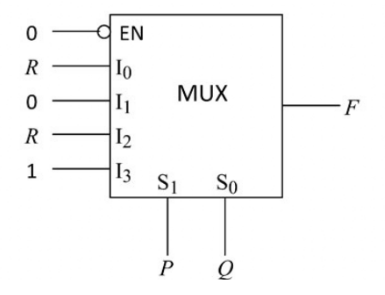
\includegraphics[width=0.6\columnwidth]{figs/Q10.png}
        \caption*{}
        \label{fig:q10}
    \end{figure}
    \begin{enumerate}
        \begin{multicols}{2}
            \item 8:23
            \item 23:8
            \item 23:31
            \item 31:23
        \end{multicols}
    \end{enumerate}
    \hfill{\brak{\text{GATE EC 2020}}}
\end{enumerate}
\begin{enumerate}
\section*{Electronics and Communication Engineering \brak{EC}}
    \item[\centerline{\textbf{Electronics and Communication Engg.}}]

    \item If $v_1, v_2, \dots, v_6$ are six vectors in $\mathbb{R}^4$, which one of the following statements is FALSE?
    \begin{enumerate}
        \item It is not necessary that these vectors span $\mathbb{R}^4$.
        \item These vectors are not linearly independent.
        \item Any four of these vectors form a basis for $\mathbb{R}^4$.
        \item If $\{v_1, v_3, v_5, v_6\}$ spans $\mathbb{R}^4$, then it forms a basis for $\mathbb{R}^4$.
    \end{enumerate}

    \hfill{\brak{\text{GATE EC 2020}}}

    \item For a vector field $\vec{A}$, which one of the following is FALSE?
    \begin{enumerate}
        \item $\vec{A}$ is solenoidal if $\nabla \cdot \vec{A} = 0$
        \item $\nabla \times \vec{A}$ is another vector field.
        \item $\vec{A}$ is irrotational if $\nabla^2 \vec{A} = 0$.
        \item $\nabla \times \brak{\nabla \times \vec{A}} = \nabla\brak{\nabla \cdot \vec{A}} - \nabla^2\vec{A}$
    \end{enumerate}

    \hfill{\brak{\text{GATE EC 2020}}}

    \item The partial derivative of the function
    \begin{center}
    $f(x,y,z) = e^{1-x \cos y} + xze^{-1/\brak{1+y^2}}$
    \end{center}
    with respect to x at the point \brak{1,0,e} is
    \begin{enumerate}
        \begin{multicols}{2}
            \item -1
            \item 0
            \item 1
            \item $\frac{1}{e}$
        \end{multicols}
    \end{enumerate}

    \hfill{\brak{\text{GATE EC 2020}}}
    
    \item The general solution of $\frac{d^2y}{dx^2} - 6\frac{dy}{dx} + 9y = 0$ is
    \begin{enumerate}
        \begin{multicols}{2}
            \item $y=C_1e^{3x} + C_2e^{-3x}$
            \item $y=\brak{C_1+C_2x}e^{-3x}$
            \item $y=\brak{C_1+C_2x}e^{3x}$
            \item $y=C_1e^{3x}$
        \end{multicols}
    \end{enumerate}

    \hfill{\brak{\text{GATE EC 2020}}}

    \item The output $y[n]$ of a discrete-time system for an input $x[n]$ is
    $$y[n] = \max_{-\infty \le k \le n} |x[k]|$$
    The unit impulse response of the system is
    \begin{enumerate}
        \item 0 for all n.
        \item 1 for all n.
        \item unit step signal $u[n]$.
        \item unit impulse signal $\delta[n]$.
    \end{enumerate}

    \hfill{\brak{\text{GATE EC 2020}}}

    \item A single crystal intrinsic semiconductor is at a temperature of 300 K with effective density of states for holes twice that of electrons. The thermal voltage is 26 mV. The intrinsic Fermi level is shifted from mid-bandgap energy level by
    \begin{enumerate}
        \begin{multicols}{2}
            \item 18.02 meV.
            \item 9.01 meV.
            \item 13.45 meV.
            \item 26.90 meV.
        \end{multicols}
    \end{enumerate}

    \hfill{\brak{\text{GATE EC 2020}}}

    \item Consider the recombination process via bulk traps in a forward biased pn homojunction diode. The maximum recombination rate is $U_{max}$. If the electron and the hole capture cross-sections are equal, which one of the following is FALSE?
    \begin{enumerate}
        \item With all other parameters unchanged, $U_{max}$ decreases if the intrinsic carrier density is reduced.
        \item $U_{max}$ occurs at the edges of the depletion region in the device.
        \item $U_{max}$ depends exponentially on the applied bias.
        \item With all other parameters unchanged, $U_{max}$ increases if the thermal velocity of the carriers increases.
    \end{enumerate}

    \hfill{\brak{\text{GATE EC 2020}}}

    \item The components in the circuit shown below are ideal. If the op-amp is in positive feedback and the input voltage $V_i$ is a sine wave of amplitude 1 V, the output voltage $V_o$ is
    \begin{figure}[H]
        \centering
        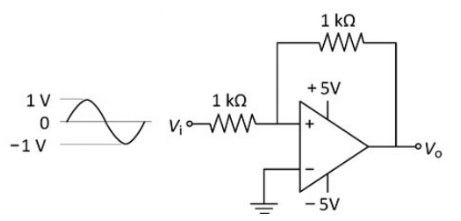
\includegraphics[width=0.6\columnwidth]{figs/Q8.png}
        \caption*{}
        \label{fig:q18}
    \end{figure}
    \begin{enumerate}
        \item a non-inverted sine wave of 2 V amplitude.
        \item an inverted sine wave of 1 V amplitude.
        \item a square wave of 5 V amplitude.
        \item a constant of either +5 V or -5 V.
    \end{enumerate}

    \hfill{\brak{\text{GATE EC 2020}}}
    
    \item In the circuit shown below, the Thevenin voltage $V_{TH}$ is
    \begin{figure}[H]
        \centering
        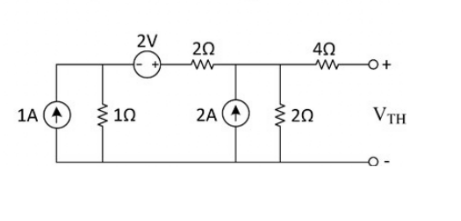
\includegraphics[width=0.5\columnwidth]{figs/Q9.png}
        \caption*{}
        \label{fig:q19}
    \end{figure}
    \begin{enumerate}
        \begin{multicols}{2}
            \item 2.4 V
            \item 2.8 V
            \item 3.6 V
            \item 4.5 V
        \end{multicols}
    \end{enumerate}

    \hfill{\brak{\text{GATE EC 2020}}}

    \item The figure below shows a multiplexer where $S_1$ and $S_0$ are the select lines, $I_0$ to $I_3$ are the input data lines, EN is the enable line, and $F(P,Q,R)$ is the output.
    \begin{figure}[H]
        \centering
        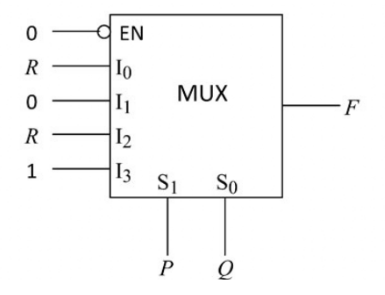
\includegraphics[width=0.4\columnwidth]{figs/Q10.png}
        \caption*{}
        \label{fig:q20}
    \end{figure}
    \begin{enumerate}
        \item $PQ+\overline{Q}R.$
        \item $P+Q\overline{R}.$
        \item $P\overline{Q}R+\overline{P}Q.$
        \item $\overline{Q}+PR.$
    \end{enumerate}

    \hfill{\brak{\text{GATE EC 2020}}}

    \item The pole-zero map of a rational function $G(s)$ is shown below. When the closed contour $\Gamma$ is mapped into the $G(s)$-plane, then the mapping encircles
    \begin{figure}[H]
        \centering
        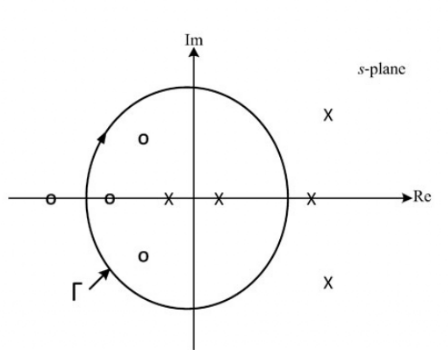
\includegraphics[width=0.4\columnwidth]{figs/Q11.png}
        \caption*{}
        \label{fig:q21}
    \end{figure}
    \begin{enumerate}
        \item the origin of the $G(s)$-plane once in the counter-clockwise direction.
        \item the origin of the $G(s)$-plane once in the clockwise direction.
        \item the point $-1+j0$ of the $G(s)$-plane once in the counter-clockwise direction.
        \item the point $-1+j0$ of the $G(s)$-plane once in the clockwise direction.
    \end{enumerate}

    \hfill{\brak{\text{GATE EC 2020}}}

    \item A digital communication system transmits a block of N bits. The probability of error in decoding a bit is $\alpha$. The error event of each bit is independent of the error events of the other bits. The received block is declared erroneous if at least one of its bits is decoded wrongly. The probability that the received block is erroneous is
    \begin{enumerate}
        \begin{multicols}{2}
            \item $N(1-\alpha)$
            \item $\alpha^N$
            \item $1-\alpha^N$
            \item $1-(1-\alpha)^N$
        \end{multicols}
    \end{enumerate}
    
    \hfill{\brak{\text{GATE EC 2020}}}

    \item The impedances $Z=jX$, for all X in the range $(-\infty, \infty)$, map to the Smith chart as
    \begin{enumerate}
        \item a circle of radius 1 with centre at (0, 0).
        \item a point at the centre of the chart.
        \item a line passing through the centre of the chart.
        \item a circle of radius 0.5 with centre at (0.5, 0).
    \end{enumerate}

    \hfill{\brak{\text{GATE EC 2020}}}

    \item Which one of the following pole-zero plots corresponds to the transfer function of an LTI system characterized by the input-output difference equation given below?
    $$y[n] = \sum_{k=0}^{3}(-1)^k x[n-k]$$
    \begin{figure}[H]
        \centering
        \begin{minipage}{0.45\textwidth}
            \centering
            (A)
            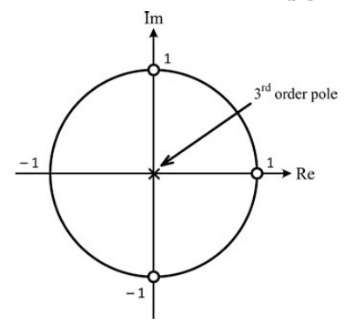
\includegraphics[width=0.8\linewidth]{figs/Q14A.png}
            \label{fig:q24a}
        \end{minipage}
        \begin{minipage}{0.45\textwidth}
            \centering
            (B)
            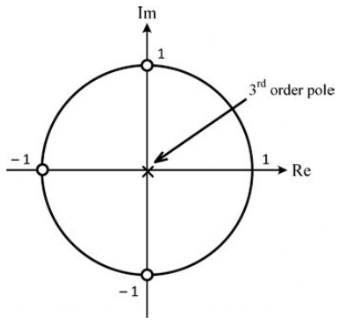
\includegraphics[width=0.8\linewidth]{figs/Q14B.png}
            \label{fig:q24b}
        \end{minipage}
        \begin{minipage}{0.45\textwidth}
            \centering
            (C)
            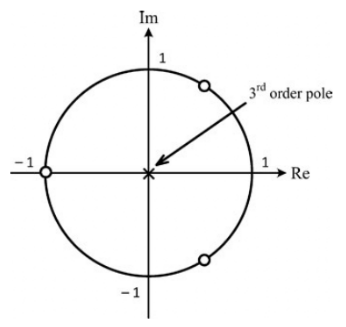
\includegraphics[width=0.8\linewidth]{figs/Q14C.png}
            \label{fig:q24c}
        \end{minipage}
        \begin{minipage}{0.45\textwidth}
            \centering
            (D)
            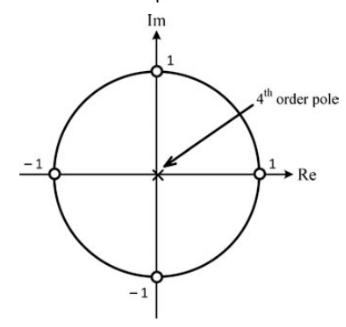
\includegraphics[width=0.8\linewidth]{figs/Q14D.png}
            \label{fig:q24d}
        \end{minipage}
    \end{figure}

    \hfill{\brak{\text{GATE EC 2020}}}

    \item In the given circuit, the two-port network has the impedance matrix $[Z] = \myvec{40 & 60 \\ 60 & 120}$. The value of $Z_L$ for which maximum power is transferred to the load is \underline{\hspace{2cm}} $\Omega$.
    \begin{figure}[H]
        \centering
        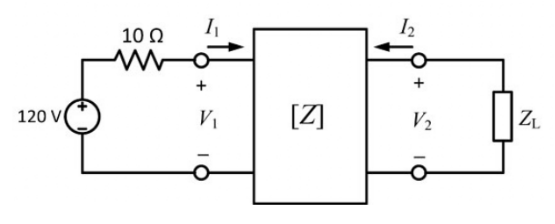
\includegraphics[width=0.7\columnwidth]{figs/Q15.png}
        \caption*{}
        \label{fig:q25}
    \end{figure}

    \hfill{\brak{\text{GATE EC 2020}}}

    \item The current in the RL-circuit shown below is $i(t)=10 \cos(5t-\pi/4)$ A. The value of the inductor (rounded off to two decimal places) is \underline{\hspace{2cm}} H.
    \begin{figure}[H]
        \centering
        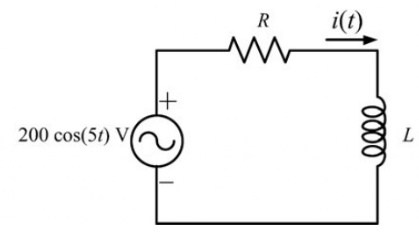
\includegraphics[width=0.5\columnwidth]{figs/Q16.png}
        \caption*{}
        \label{fig:q26}
    \end{figure}

    \hfill{\brak{\text{GATE EC 2020}}}

    \item In the circuit shown below, all the components are ideal and the input voltage is sinusoidal. The magnitude of the steady-state output $V_o$ (rounded off to two decimal places) is \underline{\hspace{2cm}} V.
    \begin{figure}[H]
        \centering
        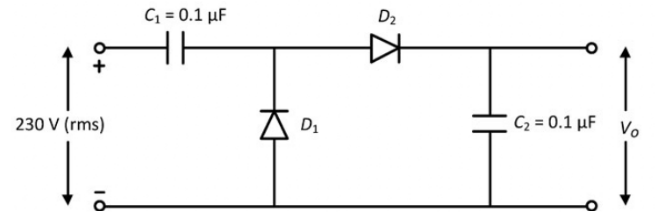
\includegraphics[width=0.8\columnwidth]{figs/Q17.png}
        \caption*{}
        \label{fig:q27}
    \end{figure}

    \hfill{\brak{\text{GATE EC 2020}}}

    \item In the circuit shown below, all the components are ideal. If $V_i$ is +2 V, the current $I_o$ sourced by the op-amp is \underline{\hspace{2cm}} mA.
    \begin{figure}[H]
        \centering
        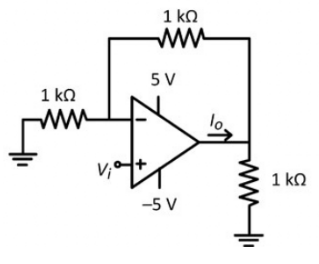
\includegraphics[width=0.4\columnwidth]{figs/Q18.png}
        \caption*{}
        \label{fig:q28}
    \end{figure}

    \hfill{\brak{\text{GATE EC 2020}}}

    \item In an 8085 microprocessor, the number of address lines required to access a 16 K byte memory bank is \underline{\hspace{2cm}}.

    \hfill{\brak{\text{GATE EC 2020}}}

    \item A 10-bit D/A converter is calibrated over the full range from 0 to 10 V. If the input to the D/A converter is 13A (in hex), the output (rounded off to three decimal places) is \underline{\hspace{2cm}} V.

    \hfill{\brak{\text{GATE EC 2020}}}

    \item A transmission line of length $3\lambda/4$ and having a characteristic impedance of 50 $\Omega$ is terminated with a load of 400 $\Omega$. The impedance (rounded off to two decimal places) seen at the input end of the transmission line is \underline{\hspace{2cm}} $\Omega$.

    \hfill{\brak{\text{GATE EC 2020}}}
    
    \item A binary random variable X takes the value +2 or -2. The probability $P(X=+2) = \alpha$. The value of $\alpha$ (rounded off to one decimal place), for which the entropy of X is maximum, is \underline{\hspace{2cm}}.

    \hfill{\brak{\text{GATE EC 2020}}}

    \item The loop transfer function of a negative feedback system is\\$$G(s)H(s) = \frac{K(s+11)}{s(s+2)(s+8)}$$\\The value of K, for which the system is marginally stable, is \underline{\hspace{2cm}}.

    \hfill{\brak{\text{GATE EC 2020}}}

    \item The random variable \\$Y = \int_{-\infty}^{\infty} W(t)\phi(t)dt$, where $\phi(t) = \begin{cases} 1; & 5 \le t \le 7 \\ 0; & \text{otherwise} \end{cases}$ \\and $W(t)$ is a real white Gaussian noise process with two-sided power spectral density $S_W(f) = 3$ W/Hz for all f. The variance of Y is \underline{\hspace{2cm}}.

    \hfill{\brak{\text{GATE EC 2020}}}

    \item The two sides of a fair coin are labelled as 0 and 1. The coin is tossed two times independently. Let M and N denote the labels corresponding to the outcomes of those tosses. For a random variable X, defined as $X = \min(M,N)$, the expected value $E(X)$ (rounded off to two decimal places) is \underline{\hspace{2cm}}.

    \hfill{\brak{\text{GATE EC 2020}}}

    \item Consider the following system of linear equations.
    \begin{align*}
        x_1 + 2x_2 &= b_1 \\
        2x_1 + 4x_2 &= b_2 \\
        3x_1 + 7x_2 &= b_3 \\
        3x_1 + 9x_2 &= b_4
    \end{align*}
    Which one of the following conditions ensures that a solution exists for the above system?
    \begin{enumerate}
        \item $b_2=2b_1$ and $6b_1 - 3b_3 + b_4 = 0$
        \item $b_3=2b_1$ and $6b_1 - 3b_3 + b_4 = 0$
        \item $b_2=2b_1$ and $3b_1 - 6b_3 + b_4 = 0$
        \item $b_3=2b_1$ and $3b_1 - 6b_3 + b_4 = 0$
    \end{enumerate}

    \hfill{\brak{\text{GATE EC 2020}}}

    \item Which one of the following options contains two solutions of the differential equation $\frac{dy}{dx} = (y-1)x$?
    \begin{enumerate}
        \item $\ln|y-1| = 0.5x^2+C$ and $y=1$
        \item $\ln|y-1| = 2x^2+C$ and $y=1$
        \item $\ln|y-1| = 0.5x^2+C$ and $y=-1$
        \item $\ln|y-1| = 2x^2+C$ and $y=-1$
    \end{enumerate}

    \hfill{\brak{\text{GATE EC 2020}}}
    
    \item The current I in the given network is
    \begin{figure}[H]
        \centering
        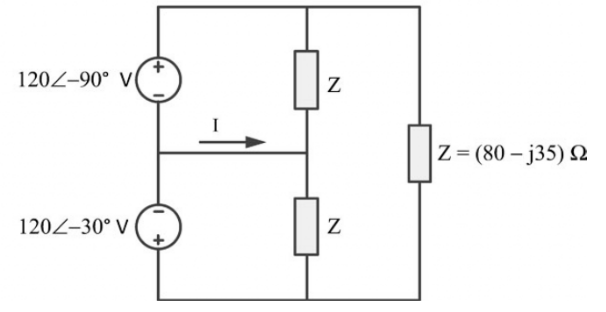
\includegraphics[width=0.5\columnwidth]{figs/Q28.png}
        \caption*{}
        \label{fig:q38}
    \end{figure}
    \begin{enumerate}
        \item 0 A.
        \item $2.38\angle-96.37^{\circ}$ A.
        \item $2.38\angle143.63^{\circ}$ A.
        \item $2.38\angle-23.63^{\circ}$ A.
    \end{enumerate}

    \hfill{\brak{\text{GATE EC 2020}}}
    
    \item A finite duration discrete-time signal $x[n]$ is obtained by sampling the continuous-time signal $x(t)=\cos(200\pi t)$ at sampling instants $t = n/400$ for $n=0, 1, \dots, 7$. The 8-point discrete Fourier transform (DFT) of $x[n]$ is defined as 
    $$X[k] = \sum_{n=0}^{7} x[n] e^{-j\frac{\pi kn}{4}}, \quad k=0,1,\dots,7$$
    Which one of the following statements is TRUE?
    \begin{enumerate}
        \item All $X[k]$ are non-zero.
        \item Only $X[4]$ is non-zero.
        \item Only $X[2]$ and $X[6]$ are non-zero.
        \item Only $X[3]$ and $X[5]$ are non-zero.
    \end{enumerate}

    \hfill{\brak{\text{GATE EC 2020}}}

    \item For the given circuit, which one of the following is the correct state equation?
    \begin{figure}[H]
        \centering
        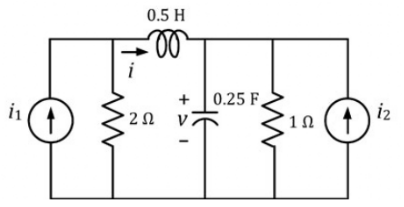
\includegraphics[width=0.6\columnwidth]{figs/Q30.png}
        \caption*{}
        \label{fig:q40}
    \end{figure}
    \begin{enumerate}
        \item $\frac{d}{dt}\myvec{v \\ i} = \myvec{-4 & 4 \\ -2 & -4}\myvec{v \\ i} + \myvec{0 & 4 \\ 4 & 0}\myvec{i_1 \\ i_2}$
        \item $\frac{d}{dt}\myvec{v \\ i} = \myvec{-4 & -4 \\ -2 & 4}\myvec{v \\ i} + \myvec{4 & 4 \\ 4 & 0}\myvec{i_1 \\ i_2}$
        \item $\frac{d}{dt}\myvec{v \\ i} = \myvec{4 & -4 \\ -2 & -4}\myvec{v \\ i} + \myvec{0 & 4 \\ 4 & 4}\myvec{i_1 \\ i_2}$
        \item $\frac{d}{dt}\myvec{v \\ i} = \myvec{-4 & -4 \\ -2 & -4}\myvec{v \\ i} + \myvec{4 & 0 \\ 0 & 4}\myvec{i_1 \\ i_2}$
    \end{enumerate}

    \hfill{\brak{\text{GATE EC 2020}}}

    \item A one-sided abrupt pn junction diode has a depletion capacitance $C_D$ of 50 pF at a reverse bias of 0.2 V. The plot of $1/C_D^2$ versus the applied voltage V for this diode is a straight line as shown in the figure below. The slope of the plot is \underline{\hspace{2cm}} $\times 10^{20} F^{-2}V^{-1}$.
    \begin{figure}[H]
        \centering
        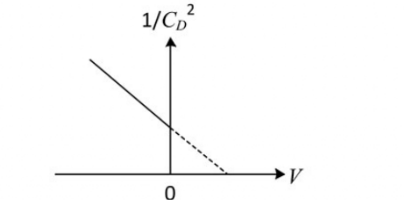
\includegraphics[width=0.3\columnwidth]{figs/Q31.png}
        \caption*{}
        \label{fig:q41}
    \end{figure}
    \begin{enumerate}
        \begin{multicols}{2}
            \item -5.7
            \item -3.8
            \item -1.2
            \item -0.4
        \end{multicols}
    \end{enumerate}

    \hfill{\brak{\text{GATE EC 2020}}}

    \item The band diagram of a p-type semiconductor with a band-gap of 1 eV is shown. Using this semiconductor, a MOS capacitor having $V_{TH}$ of -0.16 V, $C'_{ox}$ of $100 nF/cm^2$ and a metal work function of 3.87 eV is fabricated. There is no charge within the oxide. If the voltage across the capacitor is $V_{TH}$, the magnitude of depletion charge per unit area (in $C/cm^2$) is
    \begin{figure}[H]
        \centering
        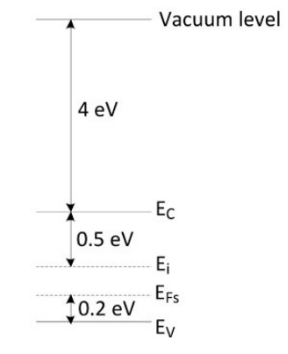
\includegraphics[width=0.4\columnwidth]{figs/Q32.png}
        \caption*{}
        \label{fig:q42}
    \end{figure}
    \begin{enumerate}
        \begin{multicols}{2}
            \item $1.70 \times 10^{-8}$
            \item $0.52 \times 10^{-8}$
            \item $1.41 \times 10^{-8}$
            \item $0.93 \times 10^{-8}$
        \end{multicols}
    \end{enumerate}
    
    \hfill{\brak{\text{GATE EC 2020}}}

    \item The base of an npn BJT T1 has a linear doping profile $N_B(x)$ as shown below. The base of another npn BJT T2 has a uniform doping $N_B$ of $10^{17} cm^{-3}$. All other parameters are identical for both the devices. Assuming that the hole density profile is the same as that of doping, the common-emitter current gain of T2 is
    \begin{figure}[H]
        \centering
        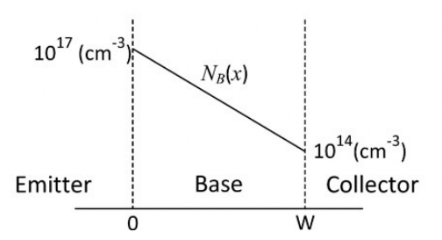
\includegraphics[width=0.6\columnwidth]{figs/Q33.png}
        \caption*{}
        \label{fig:q43}
    \end{figure}
    \begin{enumerate}
        \item approximately 2.0 times that of T1.
        \item approximately 0.3 times that of T1.
        \item approximately 2.5 times that of T1.
        \item approximately 0.7 times that of T1.
    \end{enumerate}

    \hfill{\brak{\text{GATE EC 2020}}}

    \item A pn junction solar cell of area 1.0 $cm^2$, illuminated uniformly with $100 mW cm^{-2}$, has the following parameters: Efficiency = 15\%, open circuit voltage = 0.7 V, fill factor = 0.8, and thickness = 200 $\mu$m. The charge of an electron is $1.6 \times 10^{-19}$ C. The average optical generation rate (in $cm^{-3}s^{-1}$) is
    \begin{enumerate}
        \begin{multicols}{2}
            \item $0.84 \times 10^{19}$
            \item $5.57 \times 10^{19}$
            \item $1.04 \times 10^{19}$
            \item $83.60 \times 10^{19}$
        \end{multicols}
    \end{enumerate}

    \hfill{\brak{\text{GATE EC 2020}}}

    \item For the BJT in the amplifier shown below, $V_{BE} = 0.7$ V, $kT/q = 26$ mV. Assume that BJT output resistance (ro) is very high and the base current is negligible. The capacitors are also assumed to be short circuited at signal frequencies. The input $v_i$ is direct coupled. The low frequency voltage gain $v_o/v_i$ of the amplifier is
    \begin{figure}[H]
        \centering
        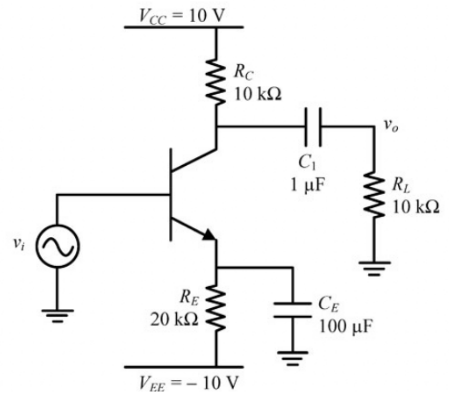
\includegraphics[width=0.4\columnwidth]{figs/Q35.png}
        \caption*{}
        \label{fig:q45}
    \end{figure}
    \begin{enumerate}
        \begin{multicols}{2}
            \item -89.42
            \item 128.21
            \item -178.85
            \item -256.42
        \end{multicols}
    \end{enumerate}

    \hfill{\brak{\text{GATE EC 2020}}}

    \item An enhancement MOSFET of threshold voltage 3 V is being used in the sample and hold circuit given below. Assume that the substrate of the MOS device is connected to -10 V. If the input voltage $V_I$ lies between $\pm 10$ V, the minimum and the maximum values of $V_G$ required for proper sampling and holding respectively, are
    \begin{figure}[H]
        \centering
        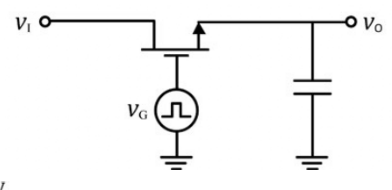
\includegraphics[width=0.4\columnwidth]{figs/Q36.png}
        \caption*{}
        \label{fig:q46}
    \end{figure}
    \begin{enumerate}
        \item 3 V and -3 V.
        \item 10 V and -10 V.
        \item 13 V and -7 V.
        \item 10 V and -13 V.
    \end{enumerate}

    \hfill{\brak{\text{GATE EC 2020}}}

    \item Using the incremental low frequency small-signal model of the MOS device, the Norton equivalent resistance of the following circuit is
    \begin{figure}[H]
        \centering
        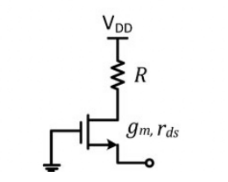
\includegraphics[width=0.4\columnwidth]{figs/Q37.png}
        \caption*{}
        \label{fig:q47}
    \end{figure}
    \begin{enumerate}
        \item $r_{ds} + R + g_m r_{ds} R$
        \item $\frac{r_{ds} + R}{1 + g_m r_{ds}}$
        \item $r_{ds} + \frac{1}{g_m} + R$
        \item $r_{ds} + R$
    \end{enumerate}

    \hfill{\brak{\text{GATE EC 2020}}}

    \item P, Q, and R are the decimal integers corresponding to the 4-bit binary number 1100 considered in signed magnitude, 1's complement, and 2's complement representations, respectively. The 6-bit 2's complement representation of $(P+Q+R)$ is
    \begin{enumerate}
        \begin{multicols}{2}
            \item 110101
            \item 110010
            \item 111101
            \item 111001
        \end{multicols}
    \end{enumerate}

    \hfill{\brak{\text{GATE EC 2020}}}

    \item The state diagram of a sequence detector is shown below. State $S_0$ is the initial state of the sequence detector. If the output is 1, then
    \begin{figure}[H]
        \centering
        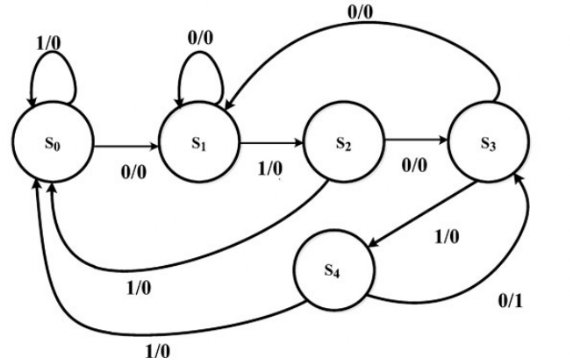
\includegraphics[width=0.8\columnwidth]{figs/Q39.png}
        \caption*{}
        \label{fig:q49}
    \end{figure}
    \begin{enumerate}
        \item the sequence 01010 is detected.
        \item the sequence 01011 is detected.
        \item the sequence 01110 is detected.
        \item the sequence 01001 is detected.
    \end{enumerate}

    \hfill{\brak{\text{GATE EC 2020}}}

    \item The characteristic equation of a system is $s^3+3s^2+(K+2)s+3K=0$. In the root locus plot for the given system, as K varies from 0 to $\infty$, the break-away or break-in point(s) lie within
    \begin{enumerate}
        \begin{multicols}{2}
            \item (-1,0).
            \item (-2,-1).
            \item (-3,-2).
            \item ($-\infty$, -3).
        \end{multicols}
    \end{enumerate}

    \hfill{\brak{\text{GATE EC 2020}}}

    \item The components in the circuit given below are ideal. If $R = 2 \text{ k}\Omega$ and $C=1 \mu F$, the -3 dB cut-off frequency of the circuit in Hz is
    \begin{figure}[H]
        \centering
        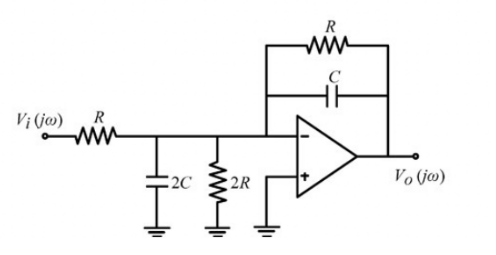
\includegraphics[width=0.6\columnwidth]{figs/Q41.png}
        \caption*{}
        \label{fig:q51}
    \end{figure}
    \begin{enumerate}
        \begin{multicols}{2}
            \item 14.92
            \item 34.46
            \item 59.68
            \item 79.58
        \end{multicols}
    \end{enumerate}

    \hfill{\brak{\text{GATE EC 2020}}}

    \item For the modulated signal $x(t) = m(t)\cos(2\pi f_c t)$, the message signal $m(t)=4 \cos(1000\pi t)$ and the carrier frequency $f_c$ is 1 MHz. The signal $x(t)$ is passed through a demodulator, as shown in the figure below. The output $y(t)$ of the demodulator is
    \begin{figure}[H]
        \centering
        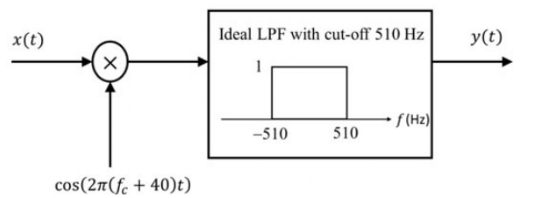
\includegraphics[width=0.8\columnwidth]{figs/Q42.png}
        \caption*{}
        \label{fig:q52}
    \end{figure}
    \begin{enumerate}
        \item $\cos(460\pi t)$.
        \item $\cos(920\pi t)$.
        \item $\cos(1000\pi t)$.
        \item $\cos(540\pi t)$.
    \end{enumerate}

    \hfill{\brak{\text{GATE EC 2020}}}

    \item For an infinitesimally small dipole in free space, the electric field $E_{\theta}$ in the far field is proportional to $(e^{-jkr}/r)\sin\theta$, where $k=2\pi/\lambda$. A vertical infinitesimally small electric dipole ($\delta l \ll \lambda$) is placed at a distance h ($h>0$) above an infinite ideal conducting plane, as shown in the figure. The minimum value of h, for which one of the maxima in the far field radiation pattern occurs at $\theta = 60^{\circ}$, is
    \begin{figure}[H]
        \centering
        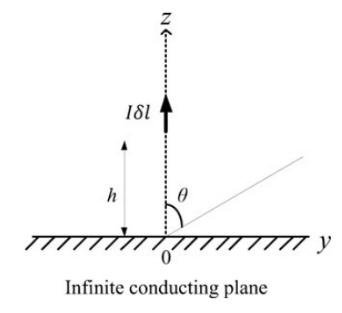
\includegraphics[width=0.4\columnwidth]{figs/Q43.png}
        \caption*{}
        \label{fig:q53}
    \end{figure}
    \begin{enumerate}
        \begin{multicols}{2}
            \item $\lambda$
            \item 0.5$\lambda$
            \item 0.25$\lambda$
            \item 0.75$\lambda$
        \end{multicols}
    \end{enumerate}

    \hfill{\brak{\text{GATE EC 2020}}}

    \item In the voltage regulator shown below, $V_I$ is the unregulated input at 15 V. Assume $V_{BE} = 0.7$ V and the base current is negligible for both the BJTs. If the regulated output $V_O$ is 9 V, the value of $R_2$ is \underline{\hspace{2cm}} $\Omega$.
    \begin{figure}[H]
        \centering
        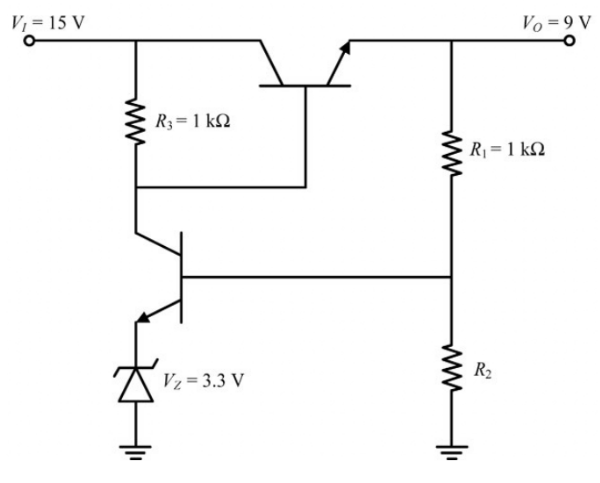
\includegraphics[width=0.6\columnwidth]{figs/Q44.png}
        \caption*{}
        \label{fig:q54}
    \end{figure}

    \hfill{\brak{\text{GATE EC 2020}}}
    
    \item The magnetic field of a uniform plane wave in vacuum is given by
    $$\vec{H}(x,y,z,t) = (\hat{a}_x + 2\hat{a}_y + b\hat{a}_z)\cos(\omega t + 3x - y - z)$$
    The value of b is \underline{\hspace{2cm}}.
    
    \hfill{\brak{\text{GATE EC 2020}}}

    \item For a 2-port network consisting of an ideal lossless transformer, the parameter $S_{21}$ (rounded off to two decimal places) for a reference impedance of 10 $\Omega$, is \underline{\hspace{2cm}}.
    \begin{figure}[H]
        \centering
        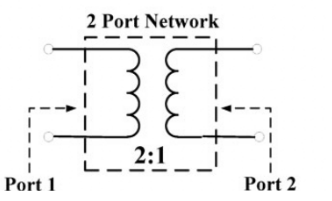
\includegraphics[width=0.4\columnwidth]{figs/Q46.png}
        \caption*{}
        \label{fig:q56}
    \end{figure}
    
    \hfill{\brak{\text{GATE EC 2020}}}

    \item $S_{PM}(t)$ and $S_{FM}(t)$ as defined below, are the phase modulated and the frequency modulated waveforms, respectively, corresponding to the message signal $m(t)$ shown in the figure.
    $$S_{PM}(t) = \cos(1000\pi t + K_p m(t))$$
    and
    $$S_{FM}(t) = \cos\left(1000\pi t + K_f \int_{-\infty}^{t} m(\tau)d\tau\right)$$
    where $K_p$ is the phase deviation constant in radians/volt and $K_f$ is the frequency deviation constant in radians/second/volt. If the highest instantaneous frequencies of $S_{PM}(t)$ and $S_{FM}(t)$ are same, then the value of the ratio $\frac{K_p}{K_f}$ is \underline{\hspace{2cm}} seconds.
    \begin{figure}[H]
        \centering
        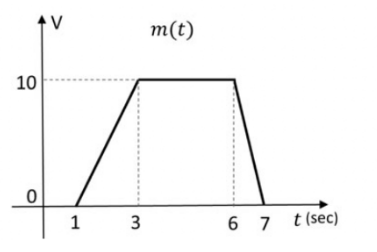
\includegraphics[width=0.5\columnwidth]{figs/Q47.png}
        \caption*{}
        \label{fig:q57}
    \end{figure}

    \hfill{\brak{\text{GATE EC 2020}}}

    \item In a digital communication system, a symbol S randomly chosen from the set $\{s_1, s_2, s_3, s_4\}$ is transmitted. It is given that $s_1 = -3$, $s_2 = -1$, $s_3 = +1$ and $s_4 = +2$. The received symbol is $Y = S+W$. W is a zero-mean unit-variance Gaussian random variable and is independent of S. $P_i$ is the conditional probability of symbol error for the maximum likelihood (ML) decoding when the transmitted symbol $S=s_i$. The index i for which the conditional symbol error probability $P_i$ is the highest is \underline{\hspace{2cm}}.

    \hfill{\brak{\text{GATE EC 2020}}}

    \item A system with transfer function $G(s) = \frac{1}{(s+1)(s+a)}$, $a>0$ is subjected to an input $5\cos(3t)$. The steady state output of the system is $\frac{1}{\sqrt{10}}\cos(3t-1.892)$. The value of a is \underline{\hspace{2cm}}.

    \hfill{\brak{\text{GATE EC 2020}}}

    \item For the components in the sequential circuit shown below, $t_{pd}$ is the propagation delay, $t_{setup}$ is the setup time, and $t_{hold}$ is the hold time. The maximum clock frequency (rounded off to the nearest integer), at which the given circuit can operate reliably, is \underline{\hspace{2cm}} MHz.
    \begin{figure}[H]
        \centering
        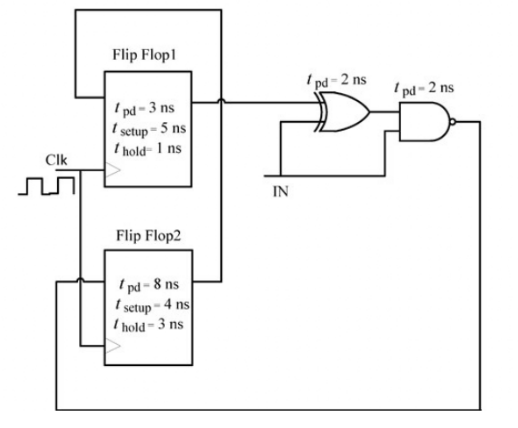
\includegraphics[width=0.8\columnwidth]{figs/Q50.png}
        \caption*{}
        \label{fig:q60}
    \end{figure}

    \hfill{\brak{\text{GATE EC 2020}}}

    \item For the solid S shown below, the value of $\iiint_S x dxdydz$ (rounded off to two decimal places) is \underline{\hspace{2cm}}.
    \begin{figure}[H]
        \centering
        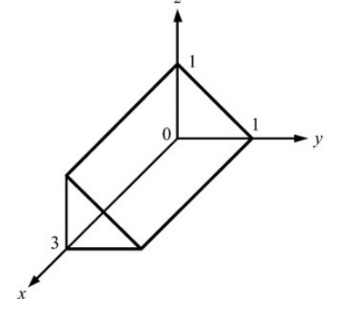
\includegraphics[width=0.4\columnwidth]{figs/Q51.png}
        \caption*{}
        \label{fig:q61}
    \end{figure}
    
    \hfill{\brak{\text{GATE EC 2020}}}

    \item $X(\omega)$ is the Fourier transform of $x(t)$ shown below. The value of $\int_{-\infty}^{\infty} |X(\omega)|^2 d\omega$ (rounded off to two decimal places) is \underline{\hspace{2cm}}.
    \begin{figure}[H]
        \centering
        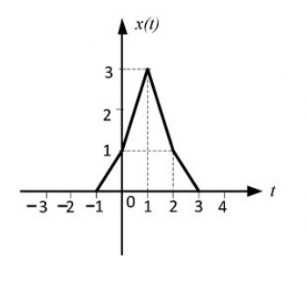
\includegraphics[width=0.4\columnwidth]{figs/Q52.png}
        \caption*{}
        \label{fig:q62}
    \end{figure}

    \hfill{\brak{\text{GATE EC 2020}}}

    \item The transfer function of a stable discrete-time LTI system is $H(z) = \frac{K(z-\alpha)}{z+0.5}$, where K and $\alpha$ are real numbers. The value of $\alpha$ (rounded off to one decimal place) with $|\alpha|>1$ for which the magnitude response of the system is constant over all frequencies, is \underline{\hspace{2cm}}.

    \hfill{\brak{\text{GATE EC 2020}}}

    \item X is a random variable with uniform probability density function in the interval $[-2, 10]$. For $Y=2X-6$, the conditional probability $P(Y \le 7 | X \ge 5)$ (rounded off to three decimal places) is \underline{\hspace{2cm}}.

    \hfill{\brak{\text{GATE EC 2020}}}

    \item Consider the following closed loop control system
    \begin{figure}[H]
        \centering
        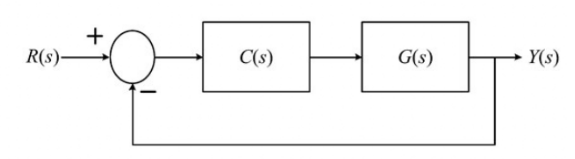
\includegraphics[width=0.6\columnwidth]{figs/Q55.png}
        \caption*{}
        \label{fig:q65}
    \end{figure}
    where $G(s) = \frac{1}{s(s+1)}$ and $C(s) = K\frac{s+1}{s+3}$. If the steady state error for a unit ramp input is 0.1, then the value of K is \underline{\hspace{2cm}}.
    
    \hfill{\brak{\text{GATE EC 2020}}}

\end{enumerate}
\end{document}

